\chapter{Experimenty}
Po dokončení jsme náš vyhledávač OsmWalk vyzkoušeli na hledání pěších tras po
Praze. Zkoumali jsme rychlost vyhledávání tras, jejich vhodnost a správnost
odhadu času a vzdálenosti. Také jsme udělali několik měření porovnávající různé
dostupné vyhledávače cest.

Každá porovnávaná trasa obsahuje popis, obrázek ukazující nalezené cesty
jednotlivých vyhledávačů a srovnání parametrů nalezených cest. Položka {\it
Vlastní měření} je naměřený čas a vzdálenost při chůzi po trase nalezené naším
vyhledávačem. 

\section{Trasa středem města}
Trasa vedoucí od Čertovky na Florenc. Trasa prochází středem města, což je hustá
zástavba bez větších volných ploch. Většina území je pěší zóna, tudíž nejsou
problémy se špatnou návazností chodníků v mapových podkladech. Vylepšení našeho
vyhledávače v podobě spojek ani zkratek by zde nemělo hrát velkou roli.
\begin{itemize}
	\item OsmWalk: 2.5\,km, 25\,min
	\item Mapy.cz: 2.7\,km, 40\,min
	\item Google maps: 2.5\,km, 31\,min
	\item OsmAnd: 2.6\,km, 30\,min
	\item Vlastní měření: 2.5\,km, 26\,min
\end{itemize}
Nalezené trasy byly přibližně stejně dlouhé a kromě Map.cz se lišily jen
minimálně. Čas Map.cz se s holedem na délku jevil jako přemrštěný, odhad délky a
času našeho vyhledávače byl přesný. 


\section{Trasa přes most Barikádníků}
Trasa vedoucí z kolejí 17.~listopadu na autobusovou zastávku Nádraží Holešovice.
Na této trase je podstatné, že hledáme trasu pro pěší a nechceme chodit po
šestiproudé magistrále. Optimální cesta používaná studenty kolejí obsahuje
několik pěšin, které nemusí být dobře zmapovány, tudíž zde je možnost využití
spojek a zkratek.

\begin{figure}[h]
	\centering
	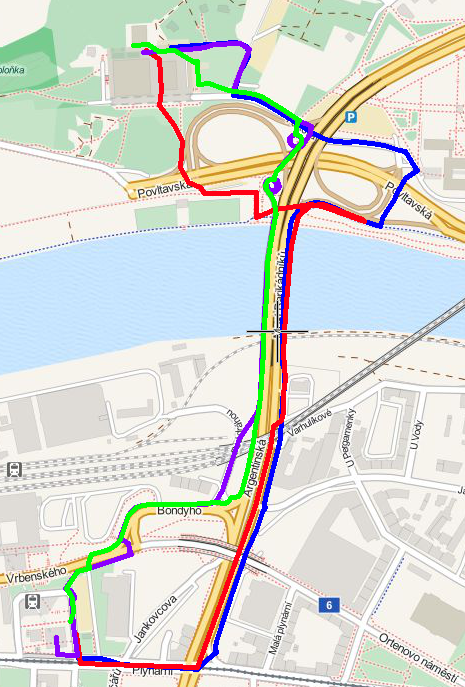
\includegraphics[width=12cm]{../img/kol-hol.png}
	\caption{Trasa přes most Barikádníků}
	\label{fig:kol-hol}
\end{figure}

\begin{itemize}
	\item OsmWalk: 1.3\,km, 14\,min
	\item Mapy.cz: 1.7\,km, 26\,min
	\item Google maps: 1.6\,km, 22\,min
	\item OsmAnd: 1.6\,km, 21\,min
	\item Vlastní měření:
\end{itemize}
Trasy nalezené jednotlivými vyhledávači se zde výrazně lišily. Podrobnější
zkoumání ukázalo, že ani Mapy.cz ani Google Maps neumí správně používat podchod
pod ulicí Povltavská. Tyto vyhledávače také přešly z chodníku na silnici,
Mapy.cz v místě, kdy už po obou stranách silnice vede chodník, Google Maps už
dříve, v místě, kde vede chodník odděleně od silnice. Naproti tomu OsmAnd našel
trasu zcela korektně po chodnících a uměl i správně použít podchod. Náš
vyhledávač našel téměř optimální trasu, problém mu dělaly rampy z podchodu na
most. Na konci naplánoval trasu po spojce mimo přechod, což ale není vadou.
%TODO Ověření odhadu.

\section{Trasa přes Petřín}
Trasa vedoucí z Malostranského náměstí na koleje Strahov. Převážná část této
trasy vede přes petřínský park, tudíž je zde potenciál pro využití zkratek. 

\begin{figure}[h]
	\centering
	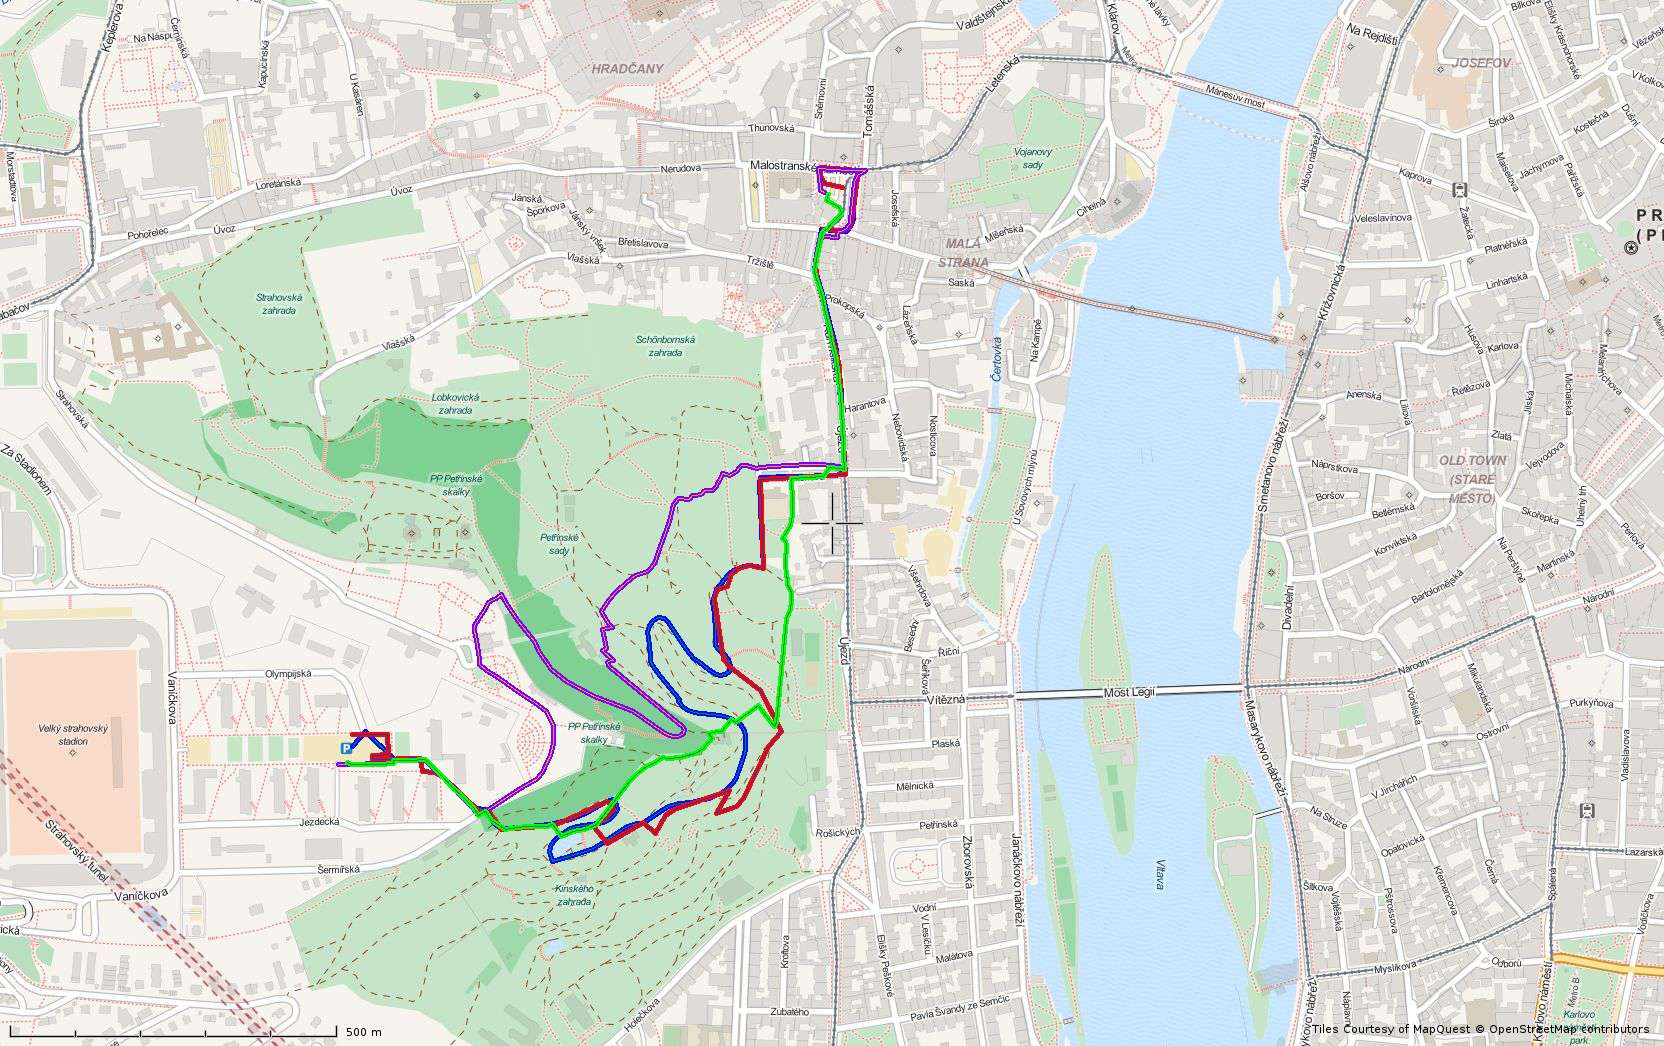
\includegraphics[width=12cm]{../img/ms-sh.png}
	\caption{Trasa přes Pteřín}
	\label{fig:kol-hol}
\end{figure}
\begin{itemize}
	\item OsmWalk: 1.7\,km, 25\,min
	\item Mapy.cz: 2.4\,km, 36\,min
	\item Google maps: 2.2\,km, 33\,min
	\item OsmAnd: 2.4\,km, 28\,min
	\item Vlastní měření: 1.8\,km, 21\,min
\end{itemize}
